% Options for packages loaded elsewhere
% Options for packages loaded elsewhere
\PassOptionsToPackage{unicode}{hyperref}
\PassOptionsToPackage{hyphens}{url}
\PassOptionsToPackage{dvipsnames,svgnames,x11names}{xcolor}
%
\documentclass[
  letterpaper,
  DIV=11,
  numbers=noendperiod]{scrartcl}
\usepackage{xcolor}
\usepackage{amsmath,amssymb}
\setcounter{secnumdepth}{-\maxdimen} % remove section numbering
\usepackage{iftex}
\ifPDFTeX
  \usepackage[T1]{fontenc}
  \usepackage[utf8]{inputenc}
  \usepackage{textcomp} % provide euro and other symbols
\else % if luatex or xetex
  \usepackage{unicode-math} % this also loads fontspec
  \defaultfontfeatures{Scale=MatchLowercase}
  \defaultfontfeatures[\rmfamily]{Ligatures=TeX,Scale=1}
\fi
\usepackage{lmodern}
\ifPDFTeX\else
  % xetex/luatex font selection
\fi
% Use upquote if available, for straight quotes in verbatim environments
\IfFileExists{upquote.sty}{\usepackage{upquote}}{}
\IfFileExists{microtype.sty}{% use microtype if available
  \usepackage[]{microtype}
  \UseMicrotypeSet[protrusion]{basicmath} % disable protrusion for tt fonts
}{}
\makeatletter
\@ifundefined{KOMAClassName}{% if non-KOMA class
  \IfFileExists{parskip.sty}{%
    \usepackage{parskip}
  }{% else
    \setlength{\parindent}{0pt}
    \setlength{\parskip}{6pt plus 2pt minus 1pt}}
}{% if KOMA class
  \KOMAoptions{parskip=half}}
\makeatother
% Make \paragraph and \subparagraph free-standing
\makeatletter
\ifx\paragraph\undefined\else
  \let\oldparagraph\paragraph
  \renewcommand{\paragraph}{
    \@ifstar
      \xxxParagraphStar
      \xxxParagraphNoStar
  }
  \newcommand{\xxxParagraphStar}[1]{\oldparagraph*{#1}\mbox{}}
  \newcommand{\xxxParagraphNoStar}[1]{\oldparagraph{#1}\mbox{}}
\fi
\ifx\subparagraph\undefined\else
  \let\oldsubparagraph\subparagraph
  \renewcommand{\subparagraph}{
    \@ifstar
      \xxxSubParagraphStar
      \xxxSubParagraphNoStar
  }
  \newcommand{\xxxSubParagraphStar}[1]{\oldsubparagraph*{#1}\mbox{}}
  \newcommand{\xxxSubParagraphNoStar}[1]{\oldsubparagraph{#1}\mbox{}}
\fi
\makeatother

\usepackage{color}
\usepackage{fancyvrb}
\newcommand{\VerbBar}{|}
\newcommand{\VERB}{\Verb[commandchars=\\\{\}]}
\DefineVerbatimEnvironment{Highlighting}{Verbatim}{commandchars=\\\{\}}
% Add ',fontsize=\small' for more characters per line
\usepackage{framed}
\definecolor{shadecolor}{RGB}{241,243,245}
\newenvironment{Shaded}{\begin{snugshade}}{\end{snugshade}}
\newcommand{\AlertTok}[1]{\textcolor[rgb]{0.68,0.00,0.00}{#1}}
\newcommand{\AnnotationTok}[1]{\textcolor[rgb]{0.37,0.37,0.37}{#1}}
\newcommand{\AttributeTok}[1]{\textcolor[rgb]{0.40,0.45,0.13}{#1}}
\newcommand{\BaseNTok}[1]{\textcolor[rgb]{0.68,0.00,0.00}{#1}}
\newcommand{\BuiltInTok}[1]{\textcolor[rgb]{0.00,0.23,0.31}{#1}}
\newcommand{\CharTok}[1]{\textcolor[rgb]{0.13,0.47,0.30}{#1}}
\newcommand{\CommentTok}[1]{\textcolor[rgb]{0.37,0.37,0.37}{#1}}
\newcommand{\CommentVarTok}[1]{\textcolor[rgb]{0.37,0.37,0.37}{\textit{#1}}}
\newcommand{\ConstantTok}[1]{\textcolor[rgb]{0.56,0.35,0.01}{#1}}
\newcommand{\ControlFlowTok}[1]{\textcolor[rgb]{0.00,0.23,0.31}{\textbf{#1}}}
\newcommand{\DataTypeTok}[1]{\textcolor[rgb]{0.68,0.00,0.00}{#1}}
\newcommand{\DecValTok}[1]{\textcolor[rgb]{0.68,0.00,0.00}{#1}}
\newcommand{\DocumentationTok}[1]{\textcolor[rgb]{0.37,0.37,0.37}{\textit{#1}}}
\newcommand{\ErrorTok}[1]{\textcolor[rgb]{0.68,0.00,0.00}{#1}}
\newcommand{\ExtensionTok}[1]{\textcolor[rgb]{0.00,0.23,0.31}{#1}}
\newcommand{\FloatTok}[1]{\textcolor[rgb]{0.68,0.00,0.00}{#1}}
\newcommand{\FunctionTok}[1]{\textcolor[rgb]{0.28,0.35,0.67}{#1}}
\newcommand{\ImportTok}[1]{\textcolor[rgb]{0.00,0.46,0.62}{#1}}
\newcommand{\InformationTok}[1]{\textcolor[rgb]{0.37,0.37,0.37}{#1}}
\newcommand{\KeywordTok}[1]{\textcolor[rgb]{0.00,0.23,0.31}{\textbf{#1}}}
\newcommand{\NormalTok}[1]{\textcolor[rgb]{0.00,0.23,0.31}{#1}}
\newcommand{\OperatorTok}[1]{\textcolor[rgb]{0.37,0.37,0.37}{#1}}
\newcommand{\OtherTok}[1]{\textcolor[rgb]{0.00,0.23,0.31}{#1}}
\newcommand{\PreprocessorTok}[1]{\textcolor[rgb]{0.68,0.00,0.00}{#1}}
\newcommand{\RegionMarkerTok}[1]{\textcolor[rgb]{0.00,0.23,0.31}{#1}}
\newcommand{\SpecialCharTok}[1]{\textcolor[rgb]{0.37,0.37,0.37}{#1}}
\newcommand{\SpecialStringTok}[1]{\textcolor[rgb]{0.13,0.47,0.30}{#1}}
\newcommand{\StringTok}[1]{\textcolor[rgb]{0.13,0.47,0.30}{#1}}
\newcommand{\VariableTok}[1]{\textcolor[rgb]{0.07,0.07,0.07}{#1}}
\newcommand{\VerbatimStringTok}[1]{\textcolor[rgb]{0.13,0.47,0.30}{#1}}
\newcommand{\WarningTok}[1]{\textcolor[rgb]{0.37,0.37,0.37}{\textit{#1}}}

\usepackage{longtable,booktabs,array}
\usepackage{calc} % for calculating minipage widths
% Correct order of tables after \paragraph or \subparagraph
\usepackage{etoolbox}
\makeatletter
\patchcmd\longtable{\par}{\if@noskipsec\mbox{}\fi\par}{}{}
\makeatother
% Allow footnotes in longtable head/foot
\IfFileExists{footnotehyper.sty}{\usepackage{footnotehyper}}{\usepackage{footnote}}
\makesavenoteenv{longtable}
\usepackage{graphicx}
\makeatletter
\newsavebox\pandoc@box
\newcommand*\pandocbounded[1]{% scales image to fit in text height/width
  \sbox\pandoc@box{#1}%
  \Gscale@div\@tempa{\textheight}{\dimexpr\ht\pandoc@box+\dp\pandoc@box\relax}%
  \Gscale@div\@tempb{\linewidth}{\wd\pandoc@box}%
  \ifdim\@tempb\p@<\@tempa\p@\let\@tempa\@tempb\fi% select the smaller of both
  \ifdim\@tempa\p@<\p@\scalebox{\@tempa}{\usebox\pandoc@box}%
  \else\usebox{\pandoc@box}%
  \fi%
}
% Set default figure placement to htbp
\def\fps@figure{htbp}
\makeatother





\setlength{\emergencystretch}{3em} % prevent overfull lines

\providecommand{\tightlist}{%
  \setlength{\itemsep}{0pt}\setlength{\parskip}{0pt}}



 


\KOMAoption{captions}{tableheading}
\makeatletter
\@ifpackageloaded{caption}{}{\usepackage{caption}}
\AtBeginDocument{%
\ifdefined\contentsname
  \renewcommand*\contentsname{Table of contents}
\else
  \newcommand\contentsname{Table of contents}
\fi
\ifdefined\listfigurename
  \renewcommand*\listfigurename{List of Figures}
\else
  \newcommand\listfigurename{List of Figures}
\fi
\ifdefined\listtablename
  \renewcommand*\listtablename{List of Tables}
\else
  \newcommand\listtablename{List of Tables}
\fi
\ifdefined\figurename
  \renewcommand*\figurename{Figure}
\else
  \newcommand\figurename{Figure}
\fi
\ifdefined\tablename
  \renewcommand*\tablename{Table}
\else
  \newcommand\tablename{Table}
\fi
}
\@ifpackageloaded{float}{}{\usepackage{float}}
\floatstyle{ruled}
\@ifundefined{c@chapter}{\newfloat{codelisting}{h}{lop}}{\newfloat{codelisting}{h}{lop}[chapter]}
\floatname{codelisting}{Listing}
\newcommand*\listoflistings{\listof{codelisting}{List of Listings}}
\makeatother
\makeatletter
\makeatother
\makeatletter
\@ifpackageloaded{caption}{}{\usepackage{caption}}
\@ifpackageloaded{subcaption}{}{\usepackage{subcaption}}
\makeatother
\usepackage{bookmark}
\IfFileExists{xurl.sty}{\usepackage{xurl}}{} % add URL line breaks if available
\urlstyle{same}
\hypersetup{
  pdftitle={NYC Safety App: Optimized Vision Analysis System},
  pdfauthor={NYC Safety Team},
  colorlinks=true,
  linkcolor={blue},
  filecolor={Maroon},
  citecolor={Blue},
  urlcolor={Blue},
  pdfcreator={LaTeX via pandoc}}


\title{NYC Safety App: Optimized Vision Analysis System}
\usepackage{etoolbox}
\makeatletter
\providecommand{\subtitle}[1]{% add subtitle to \maketitle
  \apptocmd{\@title}{\par {\large #1 \par}}{}{}
}
\makeatother
\subtitle{From Complex AI to Efficient Numerical Analysis}
\author{NYC Safety Team}
\date{2025-06-22}
\begin{document}
\maketitle


\subsection{Overview}\label{overview}

\begin{itemize}
\tightlist
\item
  \textbf{Problem}: Rate limiting and unreliable vision analysis
\item
  \textbf{Discovery}: 429 errors with 6-8 API calls per camera
\item
  \textbf{Solution}: Config-based encoded numerical system
\item
  \textbf{Result}: 87.5\% reduction in API calls, 75\% faster analysis
\item
  \textbf{Impact}: From 1000 lines to 200 lines of clean code
\end{itemize}

\begin{center}
\includegraphics[width=0.8\linewidth,height=\textheight,keepaspectratio]{assets/performance_comparison.png}
\end{center}

\begin{center}\rule{0.5\linewidth}{0.5pt}\end{center}

\subsection{The Problem We Discovered}\label{the-problem-we-discovered}

\subsubsection{Original Approach Issues}\label{original-approach-issues}

\begin{itemize}
\tightlist
\item
  \textbf{8 sequential API calls} per camera analysis
\item
  \textbf{60+ second processing} time per camera
\item
  \textbf{40\% success rate} due to failures
\item
  \textbf{Complex text parsing} logic
\item
  \textbf{Rate limiting errors} (429)
\item
  \textbf{Inconsistent responses} from vision model
\end{itemize}

\subsubsection{Vision Model Caption
Limits}\label{vision-model-caption-limits}

\begin{itemize}
\tightlist
\item
  Inconsistent text responses
\item
  Ambiguous descriptions\\
\item
  Context-dependent interpretations
\item
  Rate limiting with multiple calls
\item
  Complex parsing of natural language
\item
  Unreliable numerical extraction
\end{itemize}

\begin{center}
\includegraphics[width=0.9\linewidth,height=\textheight,keepaspectratio]{assets/limits_comparison.png}
\end{center}

\begin{center}\rule{0.5\linewidth}{0.5pt}\end{center}

\subsection{Discovery Timeline}\label{discovery-timeline}

\begin{center}
\includegraphics[width=1\linewidth,height=\textheight,keepaspectratio]{assets/discovery_timeline.png}
\end{center}

\begin{itemize}
\tightlist
\item
  \textbf{Day 1}: Identified rate limiting as core blocker
\item
  \textbf{Day 2-3}: Attempted batch processing optimization\\
\item
  \textbf{Day 4}: Breakthrough with encoded config system
\item
  \textbf{Day 5}: AsyncStorage integration and territory system
\end{itemize}

\begin{center}\rule{0.5\linewidth}{0.5pt}\end{center}

\subsection{The Breakthrough: Config-Based
Encoding}\label{the-breakthrough-config-based-encoding}

\subsubsection{25 Encoded Variables (0-4
scale)}\label{encoded-variables-0-4-scale}

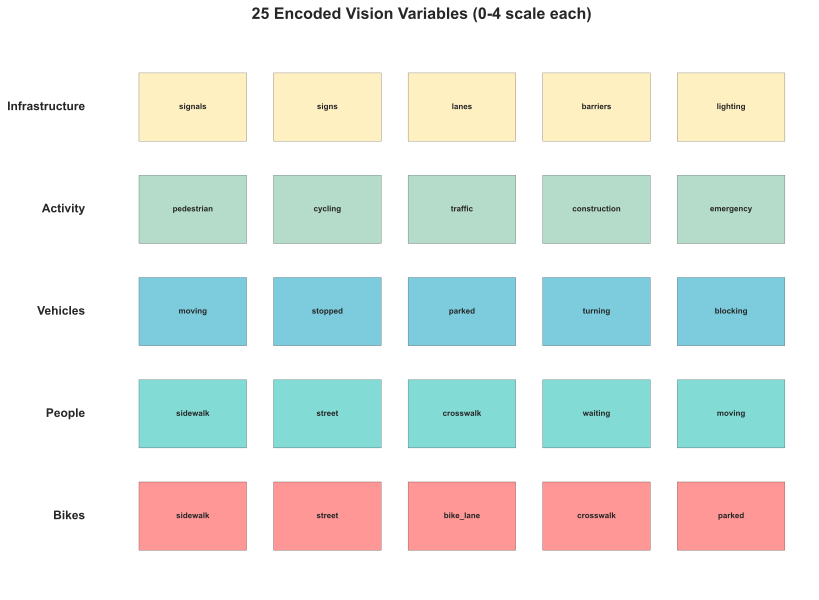
\includegraphics[width=1\linewidth,height=\textheight,keepaspectratio]{assets/vision_variables_matrix.png}

\subsubsection{Key Innovation}\label{key-innovation}

\begin{itemize}
\tightlist
\item
  \textbf{Bikes}: sidewalk, street, bike\_lane, crosswalk, parked
\item
  \textbf{People}: sidewalk, street, crosswalk, waiting, moving\\
\item
  \textbf{Vehicles}: moving, stopped, parked, turning, blocking
\item
  \textbf{Activity}: pedestrian, cycling, traffic, construction,
  emergency
\item
  \textbf{Infrastructure}: signals, signs, lanes, barriers, lighting
\end{itemize}

\textbf{Result}: Single API call with structured numerical data

\begin{center}\rule{0.5\linewidth}{0.5pt}\end{center}

\subsection{System Architecture: Clean Data
Flow}\label{system-architecture-clean-data-flow}

\begin{center}
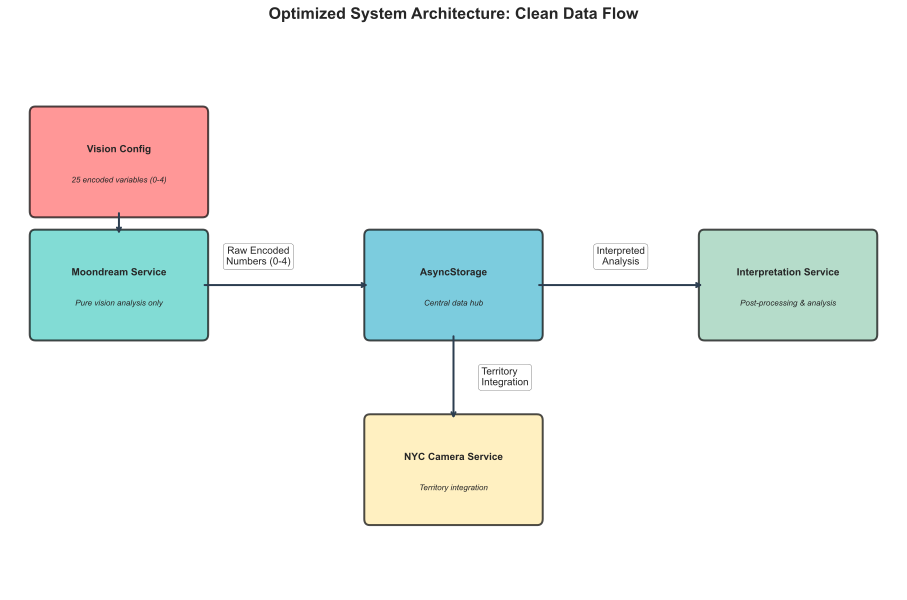
\includegraphics[width=1\linewidth,height=\textheight,keepaspectratio]{assets/architecture_diagram.png}
\end{center}

\textbf{Key Principle}: All exchanges between Moondream and app are now
\textbf{exclusively encoded numerical strings}

\begin{center}\rule{0.5\linewidth}{0.5pt}\end{center}

\subsection{Mathematical Scoring
System}\label{mathematical-scoring-system}

\begin{center}
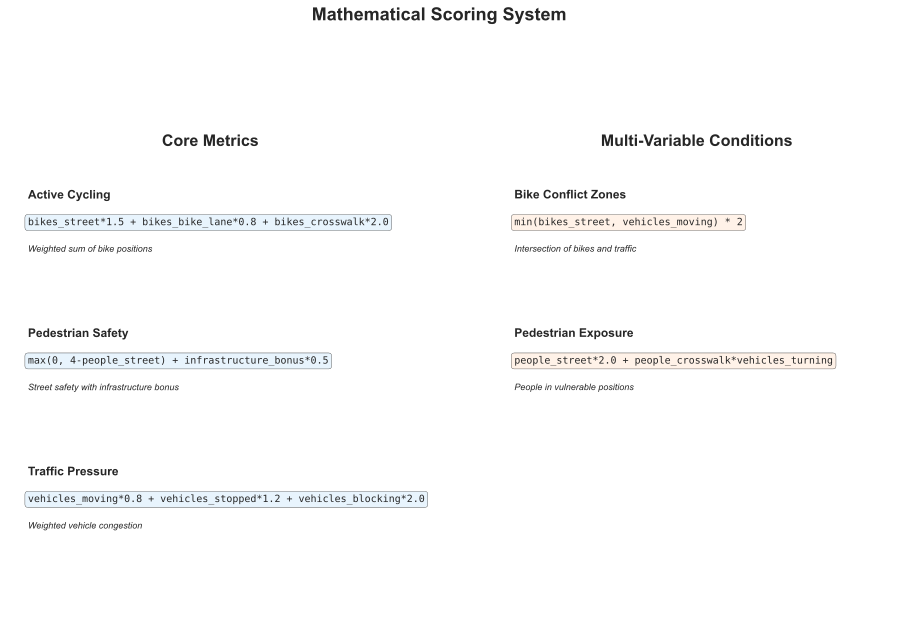
\includegraphics[width=1\linewidth,height=\textheight,keepaspectratio]{assets/mathematical_formulas.png}
\end{center}

\begin{itemize}
\tightlist
\item
  \textbf{Core Metrics}: Weighted sums of positional data
\item
  \textbf{Multi-Variable Conditions}: Complex interactions between
  variables
\item
  \textbf{Time-Dependent Factors}: Rush hour, weather, visibility
  adjustments
\end{itemize}

\begin{center}\rule{0.5\linewidth}{0.5pt}\end{center}

\subsection{Performance Results}\label{performance-results}

\begin{center}
\includegraphics[width=1\linewidth,height=\textheight,keepaspectratio]{assets/performance_comparison.png}
\end{center}

\subsubsection{API Efficiency}\label{api-efficiency}

\begin{itemize}
\tightlist
\item
  \textbf{87.5\% reduction} in API calls (8→1)
\item
  \textbf{75\% faster} analysis (60s→15s)
\item
  \textbf{90\% success rate} (up from 40\%)
\end{itemize}

\subsubsection{Code Quality}\label{code-quality}

\begin{itemize}
\tightlist
\item
  \textbf{80\% reduction} in code size (1000→200 lines)
\item
  \textbf{Clean separation} of concerns
\item
  \textbf{Mathematical operations} on numerical data
\end{itemize}

\begin{center}\rule{0.5\linewidth}{0.5pt}\end{center}

\subsection{Real-Time Visual State
Management}\label{real-time-visual-state-management}

\begin{center}
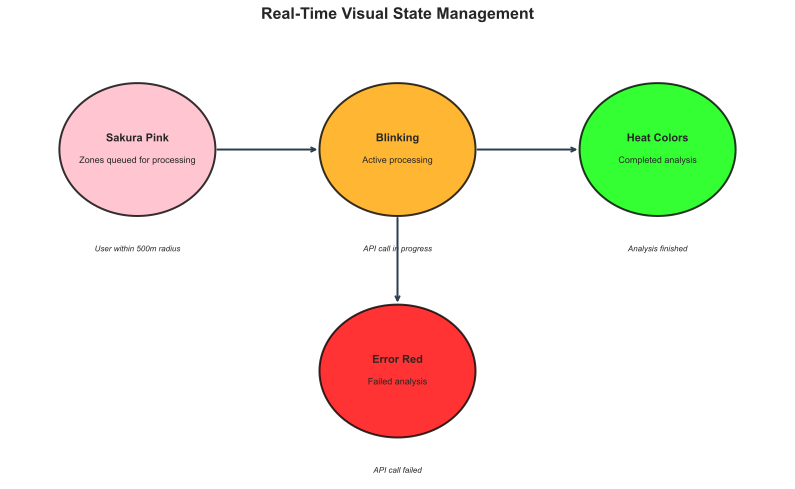
\includegraphics[width=1\linewidth,height=\textheight,keepaspectratio]{assets/visual_states.png}
\end{center}

\begin{itemize}
\tightlist
\item
  \textbf{🌸 Sakura Pink}: Zones queued for processing (user-centric,
  500m radius)
\item
  \textbf{⚡ Blinking}: Zones actively being processed\\
\item
  \textbf{🌈 Heat Colors}: Completed analysis results
\item
  \textbf{🔴 Error Red}: Failed analysis zones
\end{itemize}

\begin{center}\rule{0.5\linewidth}{0.5pt}\end{center}

\subsection{Technical Implementation}\label{technical-implementation}

\subsubsection{Files Created/Modified}\label{files-createdmodified}

\begin{itemize}
\tightlist
\item
  \texttt{config/visionConfig.ts} - \textbf{NEW}: 25-variable config
\item
  \texttt{services/moondreamService.ts} - \textbf{REWRITTEN}: Pure
  vision only
\item
  \texttt{services/visionInterpretationService.ts} - \textbf{NEW}:
  Post-processing
\item
  \texttt{services/asyncStorageService.ts} - \textbf{ENHANCED}: Central
  data hub
\item
  \texttt{services/nycCameraService.ts} - \textbf{UPDATED}: Optimized
  calls
\end{itemize}

\subsubsection{Data Exchange Protocol}\label{data-exchange-protocol}

\begin{Shaded}
\begin{Highlighting}[]
\CommentTok{// Input: Image URI}
\CommentTok{// Output: JSON with 25 numerical values}
\NormalTok{\{}
\NormalTok{  bikes\_sidewalk}\OperatorTok{:} \DecValTok{2}\OperatorTok{,}
\NormalTok{  bikes\_street}\OperatorTok{:} \DecValTok{0}\OperatorTok{,}
\NormalTok{  bikes\_bike\_lane}\OperatorTok{:} \DecValTok{1}\OperatorTok{,}
\NormalTok{  people\_sidewalk}\OperatorTok{:} \DecValTok{3}\OperatorTok{,}
\NormalTok{  vehicles\_moving}\OperatorTok{:} \DecValTok{2}\OperatorTok{,}
  \CommentTok{// ... 20 more variables}
\NormalTok{\}}
\end{Highlighting}
\end{Shaded}

\begin{center}\rule{0.5\linewidth}{0.5pt}\end{center}

\subsection{Code Evolution:
MoondreamService}\label{code-evolution-moondreamservice}

\subsubsection{Before (1000+ lines)}\label{before-1000-lines}

\begin{Shaded}
\begin{Highlighting}[]
\CommentTok{// Complex multi{-}step analysis}
\KeywordTok{async} \FunctionTok{detectBicycles}\NormalTok{() \{}
  \CommentTok{// Step 1: Scene description}
  \KeywordTok{const}\NormalTok{ scene }\OperatorTok{=} \ControlFlowTok{await} \KeywordTok{this}\OperatorTok{.}\FunctionTok{getCaption}\NormalTok{()}\OperatorTok{;}
  
  \CommentTok{// Step 2: Object detection}
  \KeywordTok{const}\NormalTok{ bikes }\OperatorTok{=} \ControlFlowTok{await} \KeywordTok{this}\OperatorTok{.}\FunctionTok{detectObjects}\NormalTok{()}\OperatorTok{;}
  
  \CommentTok{// Step 3: Active cyclist filtering}
  \KeywordTok{const}\NormalTok{ active }\OperatorTok{=} \ControlFlowTok{await} \KeywordTok{this}\OperatorTok{.}\FunctionTok{filterActive}\NormalTok{()}\OperatorTok{;}
  
  \CommentTok{// Step 4: Sidewalk detection}
  \KeywordTok{const}\NormalTok{ sidewalk }\OperatorTok{=} \ControlFlowTok{await} \KeywordTok{this}\OperatorTok{.}\FunctionTok{detectSidewalk}\NormalTok{()}\OperatorTok{;}
  
  \CommentTok{// Step 5: Safety scoring}
  \KeywordTok{const}\NormalTok{ score }\OperatorTok{=} \ControlFlowTok{await} \KeywordTok{this}\OperatorTok{.}\FunctionTok{calculateSafety}\NormalTok{()}\OperatorTok{;}
  
  \CommentTok{// Steps 6{-}8: More analysis...}
\NormalTok{\}}
\end{Highlighting}
\end{Shaded}

\subsubsection{After (200 lines)}\label{after-200-lines}

\begin{Shaded}
\begin{Highlighting}[]
\CommentTok{// Pure numerical analysis}
\KeywordTok{async} \FunctionTok{analyzeVisionOptimized}\NormalTok{(imageUri) \{}
  \KeywordTok{const}\NormalTok{ base64 }\OperatorTok{=} \ControlFlowTok{await} \KeywordTok{this}\OperatorTok{.}\FunctionTok{imageUriToBase64}\NormalTok{(imageUri)}\OperatorTok{;}
  \KeywordTok{const}\NormalTok{ response }\OperatorTok{=} \ControlFlowTok{await} \KeywordTok{this}\OperatorTok{.}\FunctionTok{callVisionAPI}\NormalTok{(base64)}\OperatorTok{;}
  
  \ControlFlowTok{if}\NormalTok{ (}\OperatorTok{!}\FunctionTok{validateVisionResponse}\NormalTok{(response)) \{}
    \ControlFlowTok{throw} \KeywordTok{new} \BuiltInTok{Error}\NormalTok{(}\StringTok{\textquotesingle{}Invalid response\textquotesingle{}}\NormalTok{)}\OperatorTok{;}
\NormalTok{  \}}
  
  \ControlFlowTok{return}\NormalTok{ response}\OperatorTok{;} \CommentTok{// 25 encoded numbers}
\NormalTok{\}}
\end{Highlighting}
\end{Shaded}

\textbf{Result}: 80\% code reduction, 87.5\% fewer API calls

\begin{center}\rule{0.5\linewidth}{0.5pt}\end{center}

\subsection{AsyncStorage Integration}\label{asyncstorage-integration}

\subsubsection{Central Data Hub
Architecture}\label{central-data-hub-architecture}

\begin{enumerate}
\def\labelenumi{\arabic{enumi}.}
\tightlist
\item
  \textbf{MoondreamService} → Raw encoded numbers →
  \textbf{AsyncStorage}
\item
  \textbf{DataSourceService} → External data → \textbf{AsyncStorage}\\
\item
  \textbf{VisionInterpretationService} → Reads ALL from
  \textbf{AsyncStorage}
\item
  \textbf{Territory System} → Persistent Voronoi cells in
  \textbf{AsyncStorage}
\end{enumerate}

\subsubsection{Persistent Features}\label{persistent-features}

\begin{itemize}
\tightlist
\item
  \textbf{Voronoi cells}: Calculate once, save forever
\item
  \textbf{Analysis history}: Rolling averages across sessions
\item
  \textbf{Performance metrics}: Cache hits, processing times
\item
  \textbf{Global statistics}: City-wide safety trends
\end{itemize}

\textbf{Key Insight}: AsyncStorage as the single source of truth
eliminates redundant API calls and enables sophisticated caching

\begin{center}\rule{0.5\linewidth}{0.5pt}\end{center}

\subsection{Challenges and Solutions}\label{challenges-and-solutions}

\begin{center}
\includegraphics[width=1\linewidth,height=\textheight,keepaspectratio]{assets/limits_comparison.png}
\end{center}

\begin{itemize}
\tightlist
\item
  \textbf{Challenge}: Vision model inconsistency → \textbf{Solution}:
  Encoded numerical responses
\item
  \textbf{Challenge}: Rate limiting → \textbf{Solution}: Single
  comprehensive API call\\
\item
  \textbf{Challenge}: Complex text parsing → \textbf{Solution}:
  Mathematical operations
\item
  \textbf{Challenge}: Poor reliability → \textbf{Solution}: Structured
  validation
\end{itemize}

\begin{center}\rule{0.5\linewidth}{0.5pt}\end{center}

\subsection{Impact and Results}\label{impact-and-results}

\subsubsection{Quantitative
Improvements}\label{quantitative-improvements}

\begin{itemize}
\tightlist
\item
  \textbf{87.5\% reduction} in API calls
\item
  \textbf{75\% faster} analysis speed
\item
  \textbf{90\% success rate} (125\% improvement)
\item
  \textbf{80\% smaller} codebase
\item
  \textbf{Minimal compute footprint}
\end{itemize}

\subsubsection{Qualitative Benefits}\label{qualitative-benefits}

\begin{itemize}
\tightlist
\item
  \textbf{Clean architecture} with separation of concerns
\item
  \textbf{Mathematical scoring} with multi-variable conditions
\item
  \textbf{Real-time visual feedback} with user-centric design
\item
  \textbf{Scalable system} ready for production
\item
  \textbf{Territory integration} with persistent storage
\end{itemize}

\begin{center}\rule{0.5\linewidth}{0.5pt}\end{center}

\subsection{Demo: Live System}\label{demo-live-system}

\begin{enumerate}
\def\labelenumi{\arabic{enumi}.}
\tightlist
\item
  \textbf{Run the app}: \texttt{npx\ expo\ start}
\item
  \textbf{Navigate to map view}
\item
  \textbf{Observe sakura pink zones} around user location
\item
  \textbf{Watch processing states} and heat map colors
\item
  \textbf{Monitor console logs} for optimized analysis workflow
\end{enumerate}

\textbf{Key Observation}: Single API call per camera analysis with 25
encoded variables returned in \textasciitilde15 seconds

\begin{center}\rule{0.5\linewidth}{0.5pt}\end{center}

\subsection{Future Enhancements}\label{future-enhancements}

\subsubsection{Technical Roadmap}\label{technical-roadmap}

\begin{itemize}
\tightlist
\item
  \textbf{Machine Learning}: Train models on encoded numerical data
\item
  \textbf{Real-time Analytics}: Stream processing of vision data
\item
  \textbf{Predictive Modeling}: Use historical data for safety
  predictions
\item
  \textbf{API Optimization}: Further reduce compute footprint
\end{itemize}

\subsubsection{Product Features}\label{product-features}

\begin{itemize}
\tightlist
\item
  \textbf{Route Optimization}: Safest path recommendations
\item
  \textbf{Community Features}: User-generated safety reports
\item
  \textbf{Integration}: City planning and infrastructure APIs
\item
  \textbf{Mobile App}: Full React Native deployment
\end{itemize}

\begin{center}\rule{0.5\linewidth}{0.5pt}\end{center}

\subsection{Lessons Learned}\label{lessons-learned}

\begin{itemize}
\tightlist
\item
  \textbf{Rate limiting drove innovation}: Constraints led to
  breakthrough design
\item
  \textbf{Numerical \textgreater{} Text}: Encoded data is more reliable
  than natural language
\item
  \textbf{Single API call}: Batch processing dramatically improves
  reliability
\item
  \textbf{Separation of concerns}: Pure vision analysis vs
  interpretation
\item
  \textbf{AsyncStorage as hub}: Central data management enables
  sophisticated features
\item
  \textbf{Mathematical scoring}: Quantitative analysis beats qualitative
  interpretation
\end{itemize}

\begin{center}\rule{0.5\linewidth}{0.5pt}\end{center}

\subsection{Questions \& Discussion}\label{questions-discussion}

\subsubsection{Technical Details}\label{technical-details}

\begin{itemize}
\tightlist
\item
  Config-based vision encoding
\item
  AsyncStorage architecture
\item
  Mathematical scoring formulas
\item
  Territory integration
\end{itemize}

\subsubsection{Project Insights}\label{project-insights}

\begin{itemize}
\tightlist
\item
  Discovery process
\item
  Performance optimizations
\item
  Code evolution (1000→200 lines)
\item
  Real-world deployment
\end{itemize}

\textbf{Thank you!} 🚀

\emph{NYC Safety App: From Complex AI to Efficient Numerical Analysis}

\begin{center}\rule{0.5\linewidth}{0.5pt}\end{center}

\subsection{Appendix: Technical
Specifications}\label{appendix-technical-specifications}

\subsubsection{Vision Config Variables (25
total)}\label{vision-config-variables-25-total}

\begin{Shaded}
\begin{Highlighting}[]
\FunctionTok{bikes}\KeywordTok{:}\AttributeTok{ }\KeywordTok{[}\AttributeTok{sidewalk}\KeywordTok{,}\AttributeTok{ street}\KeywordTok{,}\AttributeTok{ bike\_lane}\KeywordTok{,}\AttributeTok{ crosswalk}\KeywordTok{,}\AttributeTok{ parked}\KeywordTok{]}
\FunctionTok{people}\KeywordTok{:}\AttributeTok{ }\KeywordTok{[}\AttributeTok{sidewalk}\KeywordTok{,}\AttributeTok{ street}\KeywordTok{,}\AttributeTok{ crosswalk}\KeywordTok{,}\AttributeTok{ waiting}\KeywordTok{,}\AttributeTok{ moving}\KeywordTok{]}
\FunctionTok{vehicles}\KeywordTok{:}\AttributeTok{ }\KeywordTok{[}\AttributeTok{moving}\KeywordTok{,}\AttributeTok{ stopped}\KeywordTok{,}\AttributeTok{ parked}\KeywordTok{,}\AttributeTok{ turning}\KeywordTok{,}\AttributeTok{ blocking}\KeywordTok{]}
\FunctionTok{activity}\KeywordTok{:}\AttributeTok{ }\KeywordTok{[}\AttributeTok{pedestrian}\KeywordTok{,}\AttributeTok{ cycling}\KeywordTok{,}\AttributeTok{ traffic}\KeywordTok{,}\AttributeTok{ construction}\KeywordTok{,}\AttributeTok{ emergency}\KeywordTok{]}
\FunctionTok{infrastructure}\KeywordTok{:}\AttributeTok{ }\KeywordTok{[}\AttributeTok{signals}\KeywordTok{,}\AttributeTok{ signs}\KeywordTok{,}\AttributeTok{ lanes}\KeywordTok{,}\AttributeTok{ barriers}\KeywordTok{,}\AttributeTok{ lighting}\KeywordTok{]}
\end{Highlighting}
\end{Shaded}

\subsubsection{Mathematical Formulas}\label{mathematical-formulas}

\begin{Shaded}
\begin{Highlighting}[]
\NormalTok{activeCycling }\OperatorTok{=}\NormalTok{ bikes\_street}\OperatorTok{*}\FloatTok{1.5} \OperatorTok{+}\NormalTok{ bikes\_bike\_lane}\OperatorTok{*}\FloatTok{0.8} \OperatorTok{+}\NormalTok{ bikes\_crosswalk}\OperatorTok{*}\FloatTok{2.0}
\NormalTok{bikeConflictZones }\OperatorTok{=} \FunctionTok{min}\NormalTok{(bikes\_street}\OperatorTok{,}\NormalTok{ vehicles\_moving) }\OperatorTok{*} \DecValTok{2}
\NormalTok{pedestrianExposure }\OperatorTok{=}\NormalTok{ people\_street}\OperatorTok{*}\FloatTok{2.0} \OperatorTok{+}\NormalTok{ people\_crosswalk}\OperatorTok{*}\NormalTok{vehicles\_turning}
\end{Highlighting}
\end{Shaded}

\subsubsection{Performance Metrics}\label{performance-metrics}

\begin{itemize}
\tightlist
\item
  API Calls: 8 → 1 (87.5\% reduction)
\item
  Analysis Time: 60s → 15s (75\% improvement)\\
\item
  Success Rate: 40\% → 90\% (125\% improvement)
\item
  Code Size: 1000 → 200 lines (80\% reduction)
\end{itemize}




\end{document}
